\documentclass{beamer}

\usetheme{Frankfurt}
\usecolortheme{dolphin}

\usepackage{amsmath, amssymb, amsfonts}
\usepackage[utf8]{inputenc}
\usepackage[T1]{fontenc}
\usepackage[english]{babel}

\author{Alex J. Best}
\institute{WMS Talks}
\date{4/2/2014}
\title{Riemann Hypotheses}

\begin{document}

\section{Introduction}

\frame{\titlepage}

\begin{frame}
\frametitle{In this talk:}
\tableofcontents
\end{frame}

\section{The original hypothesis}

\begin{frame}{The Riemann zeta function}
\begin{block}{Euler's work:}
\begin{itemize}
\pause \item In 1735 Euler solves the \emph{Basel problem} and finds
\[\sum_{n=1}^{\infty} \frac{1}{n^2} = \frac{\pi^2}{6}.\]
\pause \item He also discovered formulae for $\sum_{n=1}^{\infty} n^{-2k}$ in terms of the Bernoulli numbers $B_{2k}$ for all natural $k$.
\note{nowadays we see this as evaluating $\zeta(2)$.}
\pause \item In fact, a nice form for \[\sum_{n=1}^{\infty} n^{-2k-1},\] is still unknown today. %TODO check
\end{itemize}
\end{block}
\end{frame}

\begin{frame}{The Riemann zeta function}
\begin{block}{Along comes Riemann:}
\begin{columns}
\begin{column}{.45\textwidth}
\begin{itemize}
\item In 1859 Riemann, a well known analyst, publishes a paper.
\end{itemize}
\end{column}
\begin{column}{.45\textwidth}
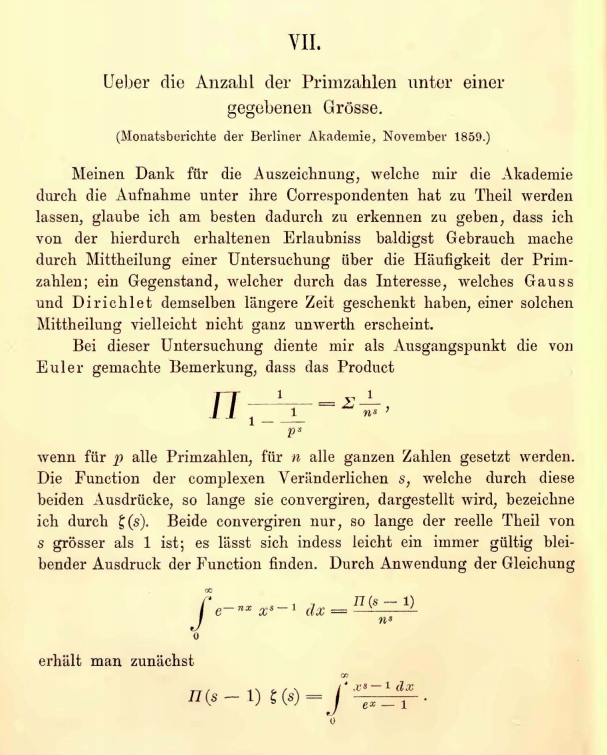
\includegraphics[width=\textwidth]{img/ueber}
\end{column}
\end{columns}
\end{block}
\end{frame}

%plots

\section{Zeta functions for graphs}

\begin{frame}{Ramanujan graphs}
\begin{block}{}
\end{block}
\end{frame}
% Sarnark wolf prize
\begin{frame}{The Ihara zeta function}
\begin{block}{}
\end{block}
\end{frame}

\section[More zetas]{More assorted zetas}

\begin{frame}{The zeta function of a scheme}
\begin{block}{}
\end{block}
\end{frame}

\section[Number theory again]{Back to number theory}
\begin{frame}{The Dedekind zeta function}
Dedekind wanted to use the 
\begin{block}{}
\end{block}
\end{frame}
\note{didn't want to talk about number theory so much as I wanted to focus more on why you might care about zeta functions even if you don't care about the structure of the primes.}

\section{Conclusion}
\begin{frame}{Conclusion}
The take away message:
\begin{itemize}
\item Zeta functions can be used to pack up useful information into one big package (a complex function).
\pause\item The properties of this package can be used to discover and prove statements about the objects you started with.
\pause\item We can also see the link different objects via their zeta functions.
\end{itemize}
\end{frame}

\end{document}
